\documentclass[a4paper]{article}
\usepackage{amsmath}
\usepackage[UTF8]{ctex}
\usepackage{tikz-feynman}
\usepackage{simplewick}
\begin{document}
    \title{在非相对论极限下电子电子相互作用的严格推导}
    \author{李成蹊\\中科院物理所}
    \date{}
    \maketitle

    采用自然单位,约定$\hbar=c=1$

    首先为了怕你电动力学基础为$0$,我给你补一点电动力学基本常识:

    我们考虑狭义相对论时空(闵可夫斯基),该空间的度规为
    \begin{equation}
        g^{\mu\nu}=g_{\mu\nu}=\begin{pmatrix}
            1\\
            &-1\\
            &&-1\\
            &&&-1
        \end{pmatrix}
    \end{equation}
    
    我们定义一个任意坐标系分量$x^\mu=(x^1,x^2,\cdots)$. 它的协变坐标为$x_\mu=(x_1,x_2,\cdots)$. 两者之间通过度规联系起来,简称为指标升降法则。
    \begin{equation}
        x_{\mu}=g_{\mu\nu}x^{\nu},x^{\mu}=g^{\mu\nu}x_{\nu}
    \end{equation}
    这里使用了爱因斯坦求和约定:$A_\mu A^\mu=\sum_{\mu}A_\mu A^\mu$. 相同指标求和。
    
    在相对论里我们定义四维坐标$x^\mu=(t,\mathbf{x})$,四维动量为$p^\mu=(E_\mathbf{p},\mathbf{p})$. 我们考虑相对论时空里运动粒子的四动量内积。四维矢量内积是一个洛伦兹常量,不会由于洛伦兹变换$\Lambda^\mu_\nu$而改变。所以四维动量内积是一个常数项,叫做质量$m$
    \begin{equation}
        p^2=p_\mu p^\mu=E_\mathbf{p}^2-|\mathbf{p}|^2=m^2
    \end{equation}
    这就是爱因斯坦著名的质能公式。我再给你进一步复习一下电动力学麦克斯韦方程:

    我们考虑闵可夫斯基空间的一个规范场(你可以理解成四维磁矢势)$A^\mu(x)=(\varphi(x),\mathbf{A}(x))$. 这里$\varphi(x)$是静电势,$\mathbf{A}(x)$是三维矢势。怕你误解,我这里提醒你,没有加粗的$x$表示四维坐标$x^\mu=(t,\mathbf{x})$. 写成底流形$\mathcal{M}$上的1-form为
    \begin{equation}
        \mathcal{A}=A_\mu dx^\mu
    \end{equation}
    我们把在四维时空的规范场$\mathcal{A}$看做是闵可夫斯基流形上的联络$\mathcal{A}$,这样可以定义曲率2-form:
    \begin{equation}
        \mathcal{F}=dA+A\wedge A
    \end{equation}
    简单做一下加减乘除可以计算出
    \begin{equation}
        \begin{split}
            \mathcal{F}&=\partial_\nu A_\mu dx^\nu\wedge dx^\mu+A_\nu A^\mu dx^\nu\wedge dx^\mu\\
            &(\mu\leftrightarrow\nu)=\frac{1}{2}(\partial_\mu A_\nu-\partial_\nu A_\mu)dx^\mu\wedge dx^\nu+[A_\mu,A_\nu]dx^\mu\wedge dx^\nu
        \end{split}
    \end{equation}
    电磁场$A^\mu(x)$满足$U(1)$规范不变性,所以电磁场理论是一个$U(1)$规范理论。$U(1)$群是一个Abel群,满足$ab=ba$. 所以上式最后一项$[A_\mu,A_\nu]=A\mu A_\nu-A_\nu A_\mu=0$. 所以我们有
    \begin{equation}
        \mathcal{F}=\frac{1}{2}F_{\mu\nu}dx^\mu dx^\nu,\quad F_{\mu\nu}=\partial_\mu A_\nu-\partial_\nu A_\mu
    \end{equation}
    这就是电磁场强$F_{\mu\nu}$的表达式。麦克斯韦方程为
    \begin{equation}
        \begin{split}
            &\partial^2 F_{\mu\nu}=J\\
            &\partial_\rho F_{\mu\nu}+\partial_\mu F_{\nu\rho}+\partial_{\nu}F_{\rho\mu}=0
        \end{split}
    \end{equation}
    为了保持洛伦兹协变性,规范场$A_\mu$满足洛伦兹规范$\partial^2A_\mu=0$. 量子化后洛伦兹规范的解满足无质量波动方程解:
    \begin{equation}
        A_\mu(x)=\int\frac{d^3p}{(2\pi)^2}\frac{1}{\sqrt{2E_{\mathbf{p}}}}\sum_{r=0}^3\left(a_{\mathbf{p}}^r\epsilon_\mu^r(p)e^{-ip\cdot x}+a_{\mathbf{p}}^{r\dagger}\epsilon_\mu^{r*}(p)e^{ip\cdot x}\right)
    \end{equation}
    这里解释一下上式意义,虽然很初等物理,但本着好心给你复习一下电动力学。$a_\mathbf{p}$和$a_{\mathbf{p}^\dagger}$分别表示湮灭、产生一个动量为$\mathbf{p}$的光子。$\epsilon_{\mu}^r(p)$表示四动量为$p$的光子极化矢量。至于如果你不知道极化矢量,你可以理解成偏振矢量。

    我们知道自由电子(没有受到任何相互作用)的拉氏量为
    \begin{equation}
        \mathcal{L}_{Dirac}=\bar{\psi}(x)(i\partial \!\!\!/-m)\psi(x)
    \end{equation}
    其中$\partial \!\!\!/=\gamma^\mu\partial_\mu$, 这里$\gamma^\mu$是Clifford代数的四维表示矩阵。你大概率在大二的时候没有学过结合代数,我这里给你科普一下Clifford代数。

    我们把满足$\{\gamma^\mu,\gamma^\nu\}=\gamma^\mu\gamma^\nu+\gamma^\nu\gamma^\mu=2g^{\mu\nu}\mathbf{1}_{4\times 4}$的集合叫做Clifford代数。其中$\{a,b\}=ab+ba$定义成Clifford乘法。对于我们现在的闵可夫斯基空间,我们可以使用Weyl表示来给出这些$\gamma^\mu$的具体表示矩阵
    \begin{equation}
        \gamma^0=\begin{pmatrix}
            0&\mathbf{1}\\
            \mathbf{1}&0
        \end{pmatrix},\quad \gamma^i=\begin{pmatrix}
            0&\sigma^i\\
            -\sigma^i&0
        \end{pmatrix}
    \end{equation}
    在电动力学里我们也知道,真空中自由电磁场拉氏量为
    \begin{equation}
        \mathcal{L}_{Maxwell}=-\frac{1}{4}F_{\mu\nu}F^{\mu\nu}
    \end{equation}
    考虑电磁场和电子之间的相互作用,我们知道他们的耦合形式是流场耦合。
    \begin{equation}
        \mathcal{L}_{int}=-e\bar\psi(x)\gamma^\mu\psi(x)A_\mu
    \end{equation}
    所以电磁场和电子相互作用拉氏量为
    \begin{equation}
        \mathcal{L}=\bar\psi(i\partial \!\!\!/-m)\psi-\frac{1}{4}F_{\mu\nu}F^{\mu\nu}-e\bar\psi\gamma^\mu\psi A_\mu
    \end{equation}
    拉氏量里不含有$\dot{\psi}$. 在大三的时候,我们学过一门课叫做理论力学。其中很大一章在讲从拉氏量到哈密顿量的变换,这个变换叫做勒让德变换:
    \begin{equation}
        H=\sum_\alpha p_\alpha\dot{q}_\alpha-L
    \end{equation}
    由于电子在电磁场里的拉氏量不含有$\dot{\psi}$,所以得到$H_{int}=-\mathcal{L}_{int}=e\bar\psi(x)\gamma^\mu\psi(x)A_\mu$.

    根据相互作用哈密顿,我们可以写出费曼规则:
    \begin{enumerate}
        \item 定点:
        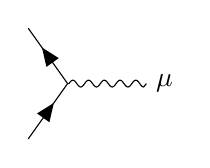
\begin{tikzpicture}
            \begin{feynman}
                \vertex (a1);
                \vertex[above=4em of a1] (a2);
                \vertex at ($(a1)!0.5!(a2) - (-0.5cm, 0)$) (a3);
                \vertex[right=1cm of a3] (a4) {\(\mu\)};
                \diagram* {
                    {[edges=fermion] (a1) -- (a3) -- (a2)},
                    (a3) -- [boson] (a4);
                };
            \end{feynman}
        \end{tikzpicture}\quad $=-ie\gamma^\mu$
        \item 光子传播子:
        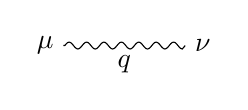
\begin{tikzpicture}
            \begin{feynman}
                \vertex (a1) {\(\mu\)};
                \vertex[right=2cm of a1] (a2) {\(\nu\)};
                \diagram*{
                    (a1) -- [boson,edge label'=\(q\)] (a2);
                };
            \end{feynman}
        \end{tikzpicture}\quad$=\frac{-ig_{\mu\nu}}{q^2+i\epsilon}$
        \item 光子外线:
        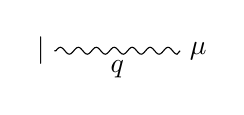
\begin{tikzpicture}
            \begin{feynman}
                \vertex (a1) {\(|\)};
                \vertex[right=2cm of a1] (a2) {\(\mu\)};
                \diagram*{
                    (a1) -- [boson,edge label'=\(q\)] (a2);
                };
            \end{feynman}
        \end{tikzpicture}\quad$=\epsilon_\mu(p)$
    \end{enumerate}
考虑电子电子的散射过程,并且考虑非相对论极限:$T$矩阵考虑微扰一阶的树图:
\begin{equation}
    i\mathcal{M}=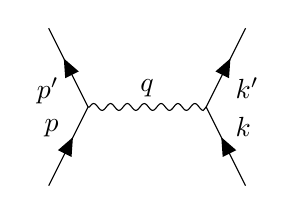
\begin{tikzpicture}
        \begin{feynman}
            \vertex (a1);
            \vertex[above=2cm of a1] (a2);
            \vertex at ($(a1)!0.5!(a2) - (-0.5cm, 0)$) (a3);
            \vertex[right=2.5cm of a1] (a4);
            \vertex[right=2.5cm of a2] (a5);
            \vertex at ($(a4)!0.5!(a5) - (0.5cm, 0)$) (a6);
            \diagram*{
                (a1) -- [fermion,edge label=\(p\)] (a3) -- [fermion,edge label=\(p'\)] (a2);
                (a3) -- [boson,edge label=\(q\)] (a6);
                (a4) -- [fermion,edge label'=\(k\)] (a6) -- [fermion,edge label'=\(k'\)] (a5);
            };
        \end{feynman}
    \end{tikzpicture}=(-ie)^2\bar{u}(p')\gamma^\mu u(p)\frac{-ig_{\mu\nu}}{q^2}\bar{u}(k')\gamma^{\nu}u(k)
\end{equation}
考虑非相对论极限下$\bar{u}(p')\gamma^0u(p)=u^\dagger(p')u(p)\simeq 2m\xi'^\dagger \xi$
\begin{equation}
    i\mathcal{M}=\frac{ie^2}{-|\mathbf{q}|^2}(2m\xi'^\dagger\xi)_p(2m\xi'^\dagger\xi)_kg_{00}
\end{equation}
在量子散射Born近似下,考虑一阶截断得到
\begin{equation}
    \langle p'|iT|p\rangle=-iV(\mathbf{q})(2\pi)\delta(E_{\mathbf{p}'}-E_{\mathbf{p}})
\end{equation}
对比上面两式得到库伦作用相互作用势的傅里叶变换$V(\mathbf{q})=e^2/|\mathbf{q}|^2$. 对$V(\mathbf{q})$做傅里叶逆变换得到$V(r)$
\begin{equation}
    \begin{split}
        V(r)&=\int\frac{d^3\mathbf{q}}{(2\pi)^3}\frac{e^2}{|\mathbf{q}|^2}e^{i\mathbf{q}\cdot\mathbf{r}}\\
        &=\frac{1}{(2\pi)^3}\int_{0}^{2\pi}d\varphi\int_0^\pi d\theta\int_0^\infty dq q^2\sin\theta\frac{e^2}{q^2}e^{iqr\cos\theta}\\
        &=\frac{e^2}{4\pi^2}\lim_{\epsilon\to 0}\int_0^\infty dq q^2\frac{e^{iqr-e^{-iqr}}}{iqr}\frac{1}{q^2+\epsilon^2}\\
        &=\frac{e^2}{4\pi^2 ir}\lim_{\epsilon\to 0}\int_{-\infty}^{\infty}dq\frac{qe^{iqr}}{q^2+\epsilon^2}\\
        &=\frac{e^2}{4\pi^2ir}\lim_{\epsilon\to 0}\int_{-\infty}^{\infty}dq\frac{qe^{iqr}}{q^2+\epsilon^2}
    \end{split}
\end{equation}
考虑如下围道
\begin{center}
    \begin{tikzpicture}
        \draw[->] (-3,0) -- (0,0) -- (3,0);
        \draw[->] (0,-3) -- (0,3);
        \draw (-0.1,1) -- (0.1,1)node[right]{$i\epsilon$};
        \draw (-0.1,-1) -- (0.1,-1)node[right]{$-i\epsilon$};
        \draw[color=red,->] (2,0) arc (0:180:2);
        \draw[color=red,->] (-2,0) -- (2,0);
    \end{tikzpicture}
\end{center}
利用留数定理计算得到
\begin{equation}
    V(r)=\frac{e^2}{4\pi^2ir}\lim_{\epsilon\to0}2\pi i \frac{e^{-\epsilon r}}{2}=\frac{e^2}{4\pi r}
\end{equation}

\end{document}